\subsection{Tutorial}
\begin{enumerate}
    \item Creare una repository su github e clonarla localmente:
    \begin{figure}[H]
    \centering
    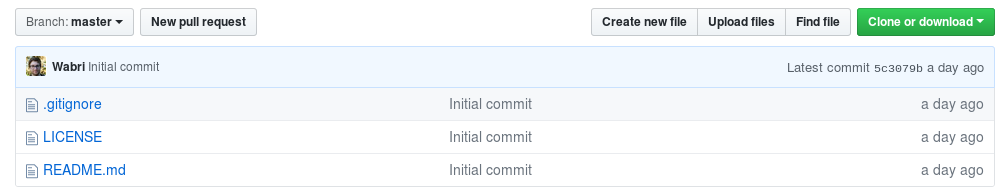
\includegraphics[width=1\linewidth]{4IntegrationWithOtherTool/tutorial/githubRepo.png}
    \end{figure}
    \item Nella repository locale creare una cartella chiamata tutorial:
    \begin{figure}[H]
    \centering
    
\includegraphics[width=0.7\linewidth]{4IntegrationWithOtherTool/tutorial/localGithubRepo.png}
    \end{figure}
    \item Spostarsi nella cartella appena creata e eseguire la build Gradle \texttt{init} per una applicazione java:
    \begin{verbatim}
        $ gradle init --type java-application
    \end{verbatim}
    \begin{figure}[H]
    \centering
    
\includegraphics[width=0.8\linewidth]{4IntegrationWithOtherTool/tutorial/gradleInit.png}
    \end{figure}
    \item Modificare il build.gradle sostituendolo con questo:
    \begin{lstlisting}[frame=single]
plugins {
    id 'java'
    id 'application'
    id 'eclipse'
}

mainClassName = 'App'

repositories {
    mavenCentral()
}

dependencies {
    testImplementation 'junit:junit:4.12'
}

task  wrapper(type: Wrapper) {
    gradleVersion = '4.6'
    distributionType = Wrapper.DistributionType.ALL
}
    \end{lstlisting}
    Con questo setting del file di build abbiamo impostato sia il plugin di eclipse sia la distribuzione del wrapper da usare.
    \item Aggiornare quindi il wrapper con la build relativa:
    \begin{verbatim}
        $ ./gradlew wrapper
    \end{verbatim}
    \item Creare i meta dati di eclipse con la build omonima definita dal plugin stesso:
    \begin{verbatim}
        $ ./gradlew eclipse
    \end{verbatim}
    \item Possiamo ora importare la repository su Eclipse:
    \begin{figure}[H]
    \centering
    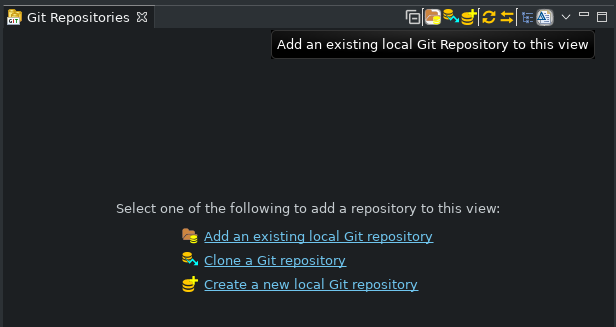
\includegraphics[width=0.8\linewidth]{4IntegrationWithOtherTool/tutorial/addExistingLocalGitRepository.png}
    \end{figure}
    \item Importare poi il progetto creato sulla repository:
    \begin{figure}[H]
    \centering
    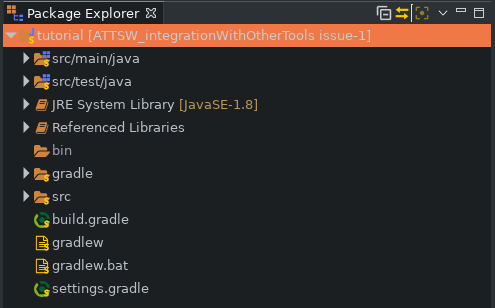
\includegraphics[width=0.8\linewidth]{4IntegrationWithOtherTool/tutorial/localRepositoryEclipse.png}
    \end{figure}
    \item Effettuare il login su \textbf{\href{https://travis-ci.org}{travis-ci.org}} e aggiungere la repository Github creata:
    \begin{figure}[H]
        \centering
        
\includegraphics{4IntegrationWithOtherTool/tutorial/newTravis.png}
    \end{figure}
    Attivare la repository:
    \begin{figure}[H]
        \centering
        
\includegraphics{4IntegrationWithOtherTool/tutorial/spuntaTravis.png}
    \end{figure}
    Andare nelle impostazioni della repository:
    \begin{figure}[H]
    \centering
    
\includegraphics{4IntegrationWithOtherTool/tutorial/settingsTravis.png}
    \end{figure}
    E indicare al server di eseguire la build solo nel caso in cui ci sia il travis.yml:
    \begin{figure}[H]
    \centering
    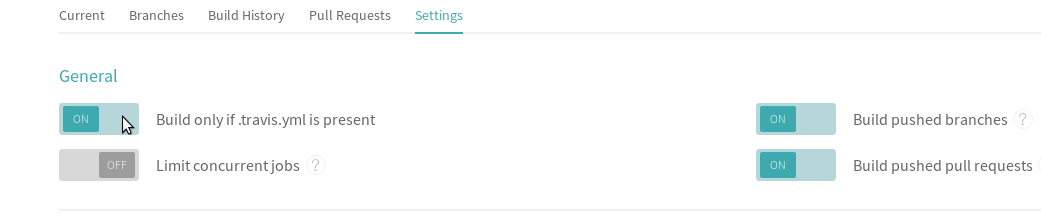
\includegraphics[width=0.7\linewidth]{4IntegrationWithOtherTool/tutorial/buildOnlyTravis.png}
    \end{figure}
    \item Creaiamo il file \texttt{travis.yml} nel quale andremo a indicare la build da eseguire, impostiamo quindi il file in questo modo:
    \begin{minted}[gobble=4, frame=single, linenos]{yaml}
    language: java

    jdk:
        - oraclejdk8
        - oraclejdk9

    # cache settings
    before_cache:
        - rm -f  $HOME/.gradle/caches/modules-2/modules-2.lock
        - rm -fr $HOME/.gradle/caches/*/plugin-resolution/
    cache:
        directories:
            - $HOME/.gradle/caches/
            - $HOME/.gradle/wrapper/

    before_script: 
        - cd tutorial

    script:
        - ./tutorial/gradlew --no-daemon -b tutorial/build.gradle test
  \end{minted}
  Salvando ed aggiornando potremmo vedere che Travis inizierà ad eseguire la build specificata nel file appena creato. Il risultato dovrebbe essere qualcosa di simile:
  \begin{figure}[H]
    \centering
    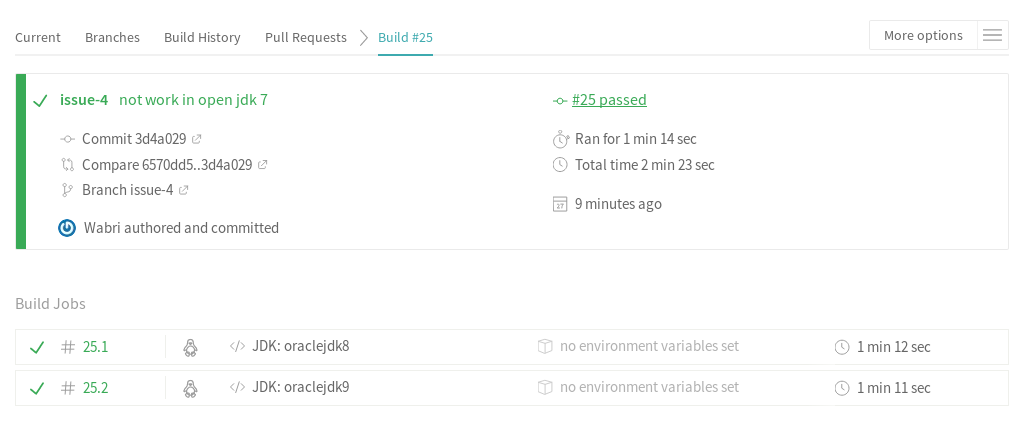
\includegraphics[width=0.9\linewidth]{4IntegrationWithOtherTool/tutorial/verifyBuild.png}
  \end{figure}
  \item Possiamo importare il tag dello stato della build nel README della repository per ottenere:
  \begin{figure}[H]
    \centering
    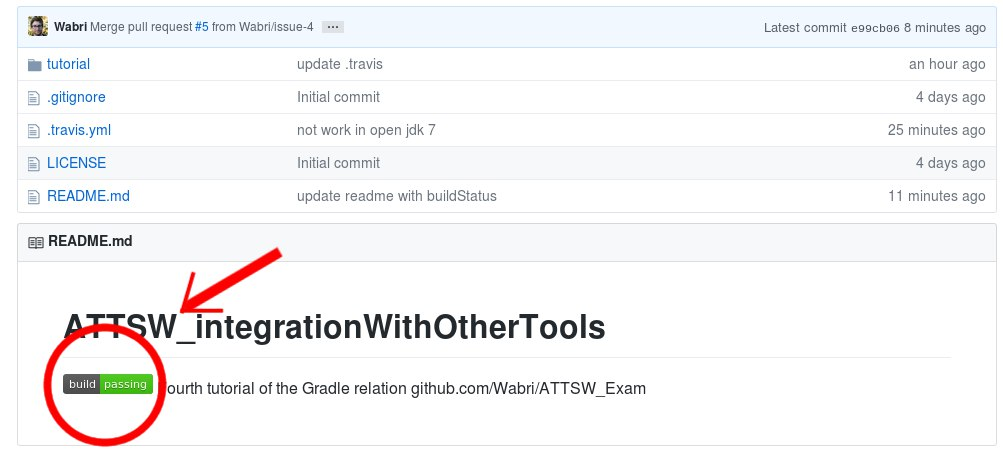
\includegraphics[width=0.8\linewidth]{4IntegrationWithOtherTool/tutorial/tagBuildPass.jpg}
  \end{figure}
  Nella build di travis accanto al nome della repository c'è questo tag:
  \begin{figure}[H]
    \centering
    
\includegraphics[width=0.2\linewidth]{4IntegrationWithOtherTool/tutorial/buildPassTag.png}
  \end{figure}
  Cliccandoci si apre una finestra in cui potrete scegliere il branch e il modo di import, nel nostro caso avremo bisogno del codice markdown. Copiamo e incolliamo direttamente nel README.md ottenendo il risultato mostrato sopra.
  \item Prima di proseguire con un esempio pratico importiamo la dipendenza Mockito utile per i test successivi:
  \begin{lstlisting}[frame=single]
dependencies {
    testImplementation 'junit:junit:4.12'
    testImplementation 'org.mockito:mockito-core:2.18.0'
}\end{lstlisting}
    \item Nei passi successivi si consiglia di creare un nuovo branch per poter vedere meglio la funzionalità di Travis. Lo schema delle classi da creare è il seguente:
    \begin{figure}[H]
    \centering
    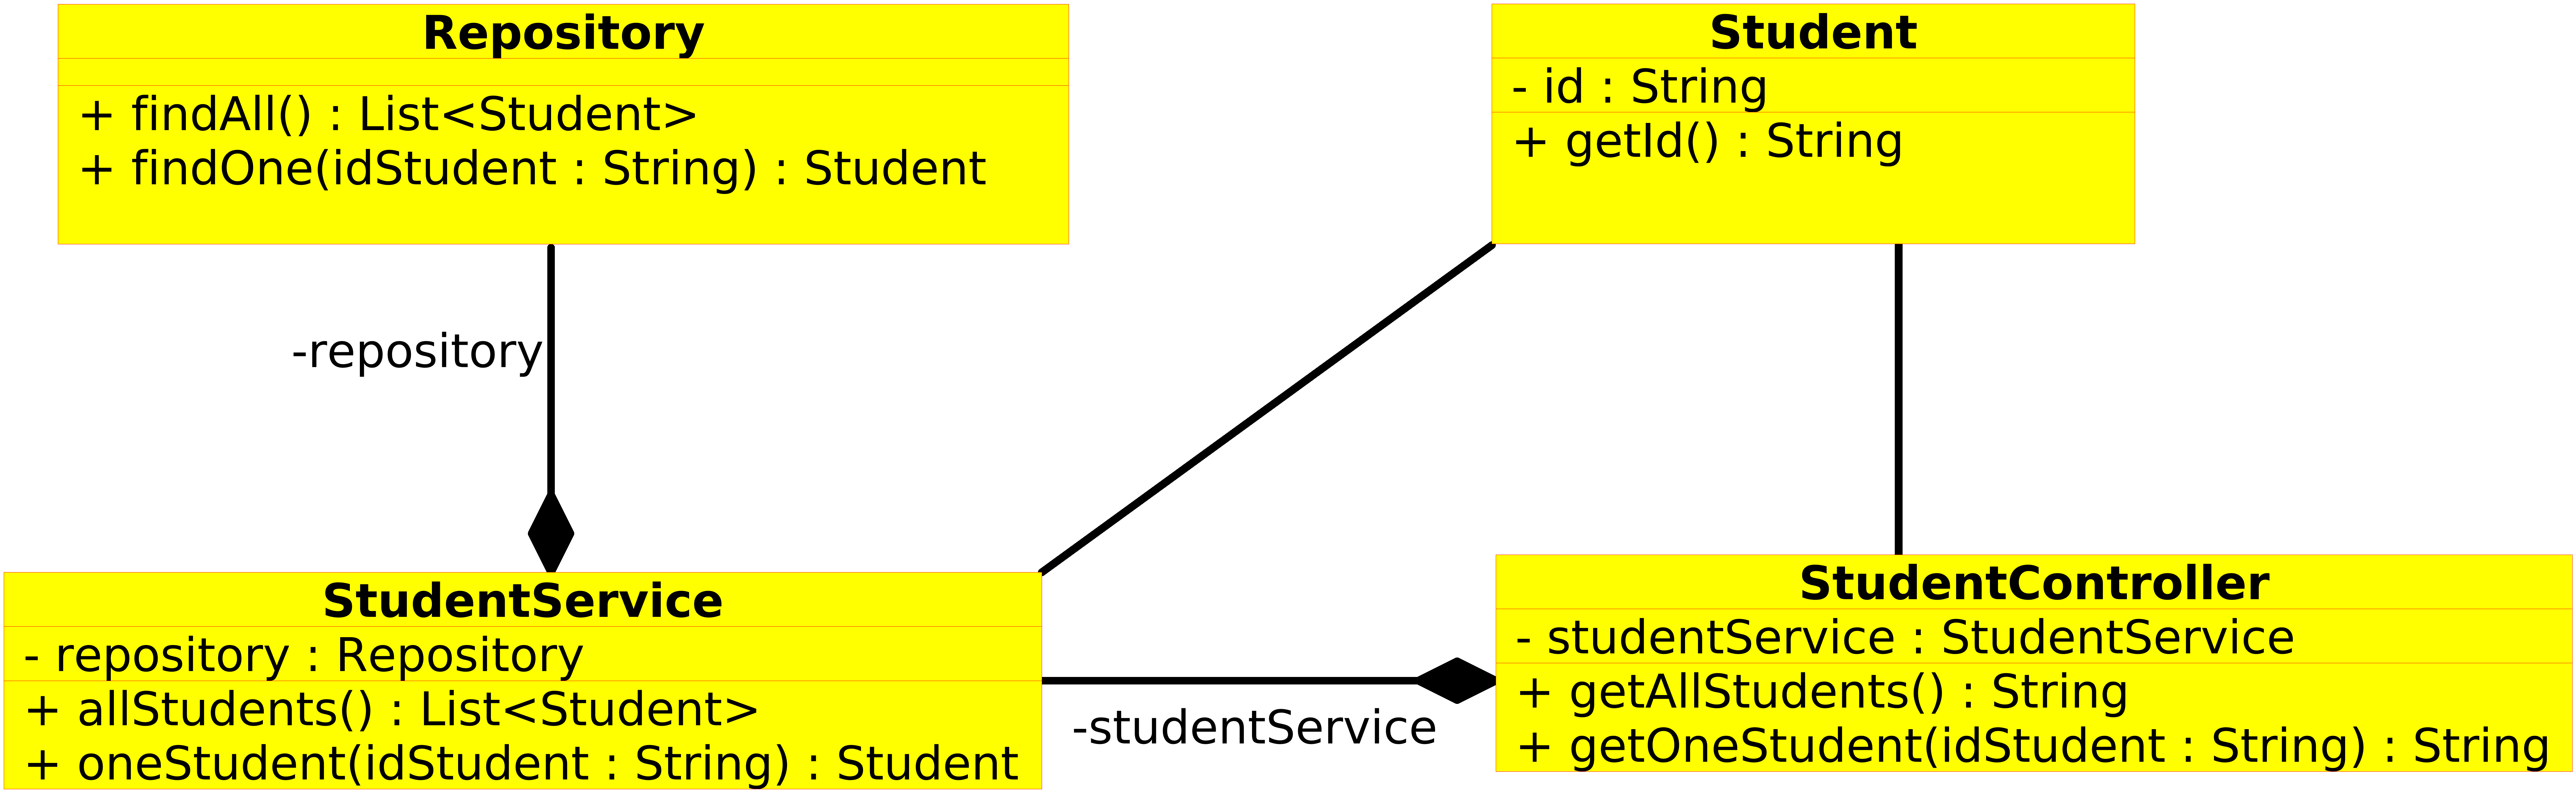
\includegraphics[width=0.8\linewidth]{4IntegrationWithOtherTool/tutorial/classDiagram.png}
  \end{figure}
\end{enumerate}